\documentclass[12pt]{article}
\usepackage{graphicx}
\usepackage{amssymb}
\usepackage{epstopdf}
\usepackage{amsmath}
\usepackage{multicol}
\usepackage{tcolorbox}
\usepackage{geometry}
\usepackage{enumitem}
\usepackage{fancyhdr}

\DeclareGraphicsRule{.tif}{png}{.png}{`convert #1 `dirname #1`/`basename #1 .tif`.png}

\textwidth = 6.5 in
\textheight = 9 in
\oddsidemargin = 0.0 in
\evensidemargin = 0.0 in
\topmargin = -23pt
\headheight = 0.0 in
\headsep = 0.0 in
\parskip = 0.2in
\parindent = 0.0in
\pagestyle{fancy}
\pagenumbering{gobble}

\newtheorem{theorem}{Theorem}
\newtheorem{corollary}[theorem]{Corollary}
\newtheorem{definition}{Definition}
%\includegraphics [height=50mm, width=50mm]{PathInt.jpg}
\title{Title} 

\begin{document}
%INSTRUCTOR NOTES

 Name:
 \begin{center}\large{2.2 Derivative at a Point}\end{center}

\textbf{Warm-up:}
In a time of $t$ seconds, a particle moves a distance of $s$ meters from its starting point, where $s=f(t)=t^2+1$. 
	\begin{enumerate}
	\item Find the average velocity between $t=2$ and $t=2.1$.
	\vfill
	\item Find the average velocity between $t=2$ and $t=2.01$.
	\vfill
	\item Find the average velocity between $t=2$ and $t=2.001$.
	\vfill
	\item Give your best estimate of the instantaneous velocity of the particle at $t=2$.
	\vfill
	\end{enumerate}


\begin{tcolorbox}
\textbf{Definitions}

The \textbf{average velocity} of an object is the change in position per unit change in time. Over time interval $a\leq t \leq b$, where $s(t)$ is the position of the object at time $t$, it is given by 
	\vspace{30mm}

\textbf{Definition of Derivative at a point:} For any function $f(t)$, we define the derivative at $t=a$, $f'(a)$, by 

\vspace{30mm}
	
	\vspace{10mm}
\end{tcolorbox}
\newpage
~
\begin{enumerate}

\item Use the limit definition of derivative to compute $f'(5) $ where $f(x)=\frac{1}{2}x+3$.
Explain why your solutions makes sense.

\vfill
\vfill
\item Use the limit definition of derivative to compute $f'(2) $ where $f(x)=\frac{1}{x}$.
Explain why your solutions makes sense.
\vfill
\vfill
\item For the function shown below, answer the following questions:\\
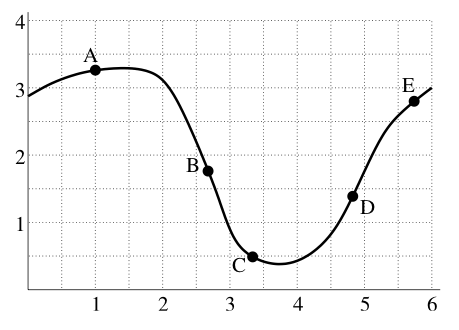
\includegraphics [scale=.75]{2_1b}
	\begin{enumerate}
	\item At what points is the slope of the curve positive?
	\vfill
	\item At what points is the slope of the curve negative?
	\vfill
	\item Rank the slopes at the 5 points in order from smallest to largest. (Note: negative values are smaller than positive values.)

	\end{enumerate}
	
\end{enumerate}
\end{document} 

%%%%%%%%%
Learning Objectives:
\begin{itemize}
\item How do we measure speed?
\item Why is the slope value a measurement of average rate of change?
\item How do we numerically compute average rate of change?
\item What is the difference between average rate of change and instantaneous rate of change?
\end{itemize}
\begin{tcolorbox}
\textbf{Warm-up: } Solve the following equations for $t$.
\begin{multicols}{2}
\begin{enumerate}
\item $(t+1)^2=9$
\item $tx+x^2=5$
\end{enumerate}
\end{multicols}
\end{tcolorbox}

MINIPAGE
\noindent\begin{minipage}{0.3\textwidth}% adapt widths of minipages to your needs
try 1
\end{minipage}%
\hspace{40mm}
\begin{minipage}{0.6\textwidth}
a) $f'(2)=$\\\

b) $f'(4)=$\\

c) $f'(6)=$\\

d) $f'(7)=$\\

e) $f'(8)=$
\end{minipage}
